\chapter{Implementierung} \label{ch:Implementierung}


Im folgenden Kapitel wird die Implementierung der Vorgehen innerhalb des Frameworks der Unreal Engine 4 behandelt. Die Baumrepräsentation enthält Daten, die von den L-System und Space Colonization Implementierungen generiert werden. Diese Daten werden an das Modellgenerierungssystem übergeben, welches die Modelldaten für eine grafische Darstellung in der Unreal Engine 4 produziert.


\section{Baumrepräsentation}  \label{sec:ImplementierungBaumrep}

Sowohl L-Systeme als auch der Space Colonization Algorithmus generieren einen graphentheoretischen Baum, auf dessen Grundlage die Modellgenerierung durchgeführt wird. Die implementierte Baumrepräsentation kann daher von beiden Systemen verwendet werden und ermöglicht es, diese mit demselben Modellgenerierungssystem zu visualisieren.

Der Baum wird durch eine Datenklasse repräsentiert, jedes Objekt dieser Klasse beschreibt einen Knoten sowie die Kante, welche vom Vorgänger zu dem Knoten führt. Die Datenklasse bietet Zugriff auf die folgenden Informationen:

\begin{description}
	\item \textbf{Vorgänger und Nachfolger:} Mithilfe eines Verweises auf den Vorgänger und eine Liste der Nachfolger eines Knotens kann der Baum-Graph vollständig repräsentiert werden. Weiterhin ermöglicht dies die Implementierung einer Reihe von rekursiven Funktionen zur Anpassung von Modelldaten.\\
	
	\item \textbf{Modell-Daten:} Kanten werden, wie in Abschnitt \ref{subsec:ZylinderMeshes} beschrieben, mithilfe von Zylindern visualisiert. Um die Generierung von Modelldaten zu vereinfachen, bietet die Datenklasse Zugriff auf Start- und Endposition, Start- und Endradius, Start- und Endnormale sowie einen Rotationswinkel. 
	
	Des Weiteren wird die Zweigtiefe des repräsentierten Knoten gespeichert.\\
	
	\item \textbf{Wachstums-Daten:} Die Wachstums-Daten bestehen aus einer Wachstumsrichtung, einem Einfluss-Zähler und dem \glqq Kein Wachstum\grqq-Zähler ($NG$-Counter), welche für den Ablauf des Space Colonization Algorithmus benötigt werden.	
\end{description}

Ein Objekt der Datenklasse kann als Astsegment eines biologischen Baumes angesehen werden und wird durch das Modellgenerierungssystem als solches visualisiert. Im Folgenden wird der Begriff \glqq Astsegment\grqq{} verwendet, um ein Objekt der Datenklasse der Baumrepräsentation zu bezeichnen.

\section{L-Systeme} \label{sec:ImplementierungLS}

Die Implementierung der Funktionsweise von L-Systemen wird durch einen Unreal-Actor verwirklicht, der im Level platziert werden kann. Nach Start des Levels wird das angegebene Axiom anhand der Produktionsregeln abgeleitet und die sich ergebende Zeichenkette von der Turtle-Implementierung interpretiert.

\subsection{Parameter}

Dem L-System-Actor werden die folgenden Parameter über die Editor-UI übergeben:

\begin{description}
	\item \textbf{Anzahl der Ableitungen:} Die Anzahl der Ableitungen in $\mathbb{N}^+$, welche auf dem Axiom durchgeführt werden. \\
	
	\item \textbf{Axiom:} Das Axiom in Form einer Zeichenkette. \\
	
	\item \textbf{Konstanten:} Eine Konstante besteht aus der Angabe eines Identifikationssymbols und eines Wertes in $\mathbb{R}$. Konstanten können im Axiom und in den Nachfolgern der Produktionen verwendet werden.\\	
	
	\item \textbf{Produktionen:} Jede Produktion besteht aus Angabe eines Vorgängers, eine Liste von Parametern und einem Nachfolger. Der Vorgänger und jeder Parameter entspricht einem einzelnen Symbol, der Nachfolger wird als Zeichenkette eingetragen. Die Parametersymbole können nur innerhalb des Nachfolgers verwendet werden. Der Vorgänger und die Liste der Parameter bilden das parametrische Wort, welches bei einer Ableitung durch den Nachfolger ersetzt wird. \\
	
	\item \textbf{Tropismus:} Der Einfluss von Tropismus in Form eines dreidimensionalen Vektors und eines Biegsamkeitsfaktors.
\end{description}
\begin{figure} [hbtp]
	\centering
	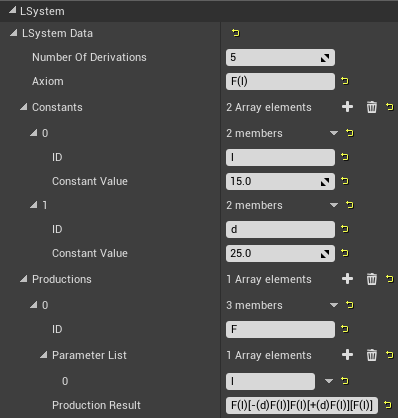
\includegraphics[height=0.4\textheight]{images/LS_ExampleUE4UI.png}
	\caption{Ein Beispiel für die Angabe des L-Systems aus Gleichung \ref{eq:ProdBranching2} mit der resultierenden Baumstruktur aus Abbildung \ref{fig:Branching2L15D25}.}
	\label{fig:LS_ExampleUE4UI}
\end{figure}
Für das Axiom und die Produktionen gelten die in Kapitel \ref{ch:LSysteme} festgelegten Regeln für die Definition von L-Systemen. Weiterhin gelten die Regeln für die Angabe von arithmetischen Operationen. Die Verwendung von Klammern ist jedoch auf die Angabe von Parametern eines parametrischen Wortes beschränkt, ihre Verwendung zur Beeinflussung der Auswertungsreihenfolge eines arithmetischen Ausdrucks wird nicht unterstützt.

Ein Beispiel für die korrekte Eingabe eines L-Systems über die Editor-UI wird in Abbildung \ref{fig:LS_ExampleUE4UI} gezeigt.

\subsection{Ableitung}

Zu Anfang der Erstellung des L-System-Actors werden alle Konstantensymbole im Axiom und den Produktionen durch die Konstantenwerte ersetzt. 

Die Implementierung arbeitet durchgehend auf derselben Zeichenkette, angefangen mit dem Axiom. In jeder Ableitung werden die in den Produktionsregeln definierten parametrischen Wörter durch die angegebenen Nachfolger ersetzt.

Nachdem die vorgegebene Anzahl von Ableitungen durchgeführt wurde, wird die resultierende Zeichenkette an die Turtle-Implementierung weiter geleitet.

\subsection{Turtle Interpretation} \label{subsec:TurtleInterpretationImplementation}

Der Turtle-Implementierung wird die aus den Ableitungen resultierende Zeichenkette übergeben. Diese wird daraufhin sequentiell abgearbeitet und entsprechend den in Abschnitt \ref{sec:LS_Baumstrukturen} vorgestellten Konzepten interpretiert. Der resultierende Baum wird für die Konstruktion des Modells an das Modellgenerierungssystem weitergegeben.

\section{Space Colonization Algorithmus} \label{sec:ImplementierungSCA}

Die Implementierung einer Space-Colonization-Algorithmus-Baumstruktur stellt sich aus der Platzierung von mindestens einem Actor für die Repräsentation des Einflussbereichs und einem Actor für die Generierungsprozedur zusammen.

\subsection{Einflussbereiche}

Durch die Platzierung von Einflussbereich-Actors kann die Verteilung von Einflusspunkten mithilfe des Unreal-Editors angepasst werden. Es sind derzeit zwei Formen von Einflussbereichen wählbar: Eine Kugel- und eine Zylinderform. Die Kugelform erfordert die Angabe eines Kugelradius während die Zylinderform durch Höhe und Radius beschrieben wird. 

Einem Space-Colonization-Actor können mehrere Einflussbereiche zugeordnet werden, um eine bestimmte Baumstruktur zu formen. Jeder Einflussbereich-Actor wird weiterhin in einem vorgegebenen Abstand zum Space-Colonization-Actor platziert.

Dem Einflussbereich muss eine positive Anzahl von zu generierenden Einflusspunkten und ein Random-Seed Wert übergeben werden. Ein Random-Seed ist ein Wert, der von einem Zufallsgenerator verwendet wird, um eine zufällig wirkende Folge von Zahlen zu generieren. Bei Verwendung desselben Random-Seeds wird dieselbe Folge von Zufallszahlen erstellt, was eine gewisse Kontrolle über die Generierung ermöglicht. Somit wird, wenn alle anderen Parameter ebenfalls übereinstimmen, mit demselben Random-Seed Wert dieselbe Baumstruktur aufgebaut. 

\subsection{Parameter}

Dem Space-Colonization-Actor werden Parameter des ursprünglichen Algorithmus sowie Eingaben für die in Abschnitt \ref{sec:SCA_Erweiterungen} besprochenen Erweiterungen über das Editor-UI übergeben. Zu den ursprünglichen Parametern gehören der Minimalradius, Einflussradius, Schrittweite, ein Tropismusvektor sowie die Anzahl der durchzuführenden Iterationen. Zu den erweiterten Parametern gehören der maximale Grad, die maximale Zweigtiefe, die maximale Anzahl von \glqq Kein Wachstum\grqq{}-Iterationen und eine Abfrage, ob gewichtetes Wachstum durchgeführt werden soll.

Weiterhin müssen die zugeordneten Einflussbereich-Actors angegeben werden -- damit der Algorithmus durchgeführt werden kann, muss mindestens einer dieser Actors mit mindestens einem Einflusspunkt eingetragen werden.

\subsection{Ablauf des Algorithmus}

Die Einflusspunkte aller dem Space-Colonization-Actor zugeordneten Einflussbereiche werden diesem zu Beginn der Baum-Generierung übergeben. Daraufhin wird ein Baum entsprechend der in Abschnitt \ref{sec:GenerierungBaumstrukturen} und Abschnitt \ref{sec:SCA_Erweiterungen} vorgestellten Konzepte aufgebaut und für die Konstruktion des Modells an das Modellgenerierungssystem weitergegeben.

\section{Modellgenerierung} \label{sec:Modellgenerierung}

L-System- und Space-Colonization-Actors übergeben dem Modellgenerierungssystem nach Ablauf der Generierung einen graphentheoretischen Baum. Das Modellgeneriungssystem erstellt daraus ein dreidimensionales Mesh (engl. für Polygonnetz) in der vom Framework geforderten Form. Das Mesh entspricht der Visualisierung der Kanten des graphentheoretischen Baums in Form von Zylindern und simuliert dadurch vereinfacht die Aststruktur eines biologischen Baumes. \cite[S.2]{SpaceColonizationAlgorithm:07} 

\subsection{Procedural Mesh Component}

Die Procedural Mesh Component ist eine Komponente der Unreal Engine, welche die Darstellung von prozedural generierten Polygonnetzen zulässt. Ein Vertex ist ein Punkt in einem Polygonnetz mit zur Visualisierung benötigten Informationen. Der Komponente werden Vertexdaten in Form von Listen aus Positions-, Normalen-, Tangenten-, Textur- und Indexdaten übergeben. Das Grafiksystem der Unreal Engine ist daraufhin in der Lage, die Komponente als dreidimensionales Modell im Level darzustellen. \cite{ProceduralMeshComponent:15} Die Vertexdaten werden, basierend auf dem übergebenen Baum und den Parametern, vom Modellgenerierungssytem erstellt.

Jedem L-System-Actor und Space-Colonization-Actor ist eine Procedural Mesh Component zugeordnet.

\subsection{Parameter} \label{subsec:Modellgenerierung_Parameter}

Dem Modellgenerierungssystem werden die folgenden Parameter über das Editor-UI übergeben:

\begin{description}
	\item \textbf{Radius-Daten:} Diese beinhalten den Blattradius, den Radiuswachstumswert, den Stammbreitenmultiplikator und die Abfrage, ob Radius\-be\-rech\-nung\-en durch\-ge\-führt werden sollen. \\
	
	\item \textbf{Genauigkeit:} Diese beinhalten die minimale und maximale Anzahl von Zylindersektionen sowie den Kurvenreduktionswert. \\
	
	\item \textbf{Sonstiges:} Weiterhin wird ein Startrotationswinkel, ein Material und eine Abfrage, ob ein fraktales Mesh erstellt werden soll, übergeben. Ein Material beinhaltet Textur- und Shaderinformationen und ist für die Oberflächenbeschaffenheit des generierten Modells verantwortlich.
\end{description}

\subsection{Operationen auf dem Baum}

Folgende Operationen werden vor Beginn der Modelldatengenerierung auf dem graphentheoretischen Baum durchgeführt:

\begin{description}
	\item \textbf{Kurvenreduktion:} Die Kurvenreduktion wird, beginnend mit dem Wurzel-Astsegment des Baums, rekursiv ausgeführt. In jedem Schritt wird überprüft ob das aktuelle Astsegment entsprechend der Beschreibung in Paragraph \ref{par:Kurvenreduktion} entfernt werden kann. Falls nicht, wird die Kurvenreduktion auf allen Nachfolgern des aktuellen Astsegment durchgeführt. Die Rekursion bricht ab, falls ein Astsegment keine Nachfolger besitzt.
	
	Der Parameter \glqq Kurvenreduktionswert\grqq{} entspricht dem Maximalwert des Skalarprodukts $max_K$.\\
	
	\item \textbf{Radiusberechnung:} Der Endradius jedes Astsegments wird, beginnend mit dem Wurzel-Astsegment des Baums, rekursiv anhand von Gleichung \ref{eq:Radiusberechnung} berechnet. Der Parameter \glqq Blattradius\grqq{} entspricht $r_0$ und der \glqq Radiuswachstumswert\grqq{} entspricht $g$. 
	
	Der Startradius jedes Astsegments wird auf den Wert des Endradius seines Vorgängers gesetzt. Da das Wurzel-Astsegment keinen Vorgänger besitzt, wird der Startradius aus der Multiplikation des Stammbreitenmultiplikators mit dem Endradius des Objekts bestimmt.\\
	
	\item \textbf{Normalenberechnung:} Normalen werden für die Berechnung der Modelldaten benötigt. Die Endnormale $\overrightarrow{n_{e}}$ jedes Astsegments wird mithilfe der Startposition $\overrightarrow{p_{s}}$ und Endposition $\overrightarrow{p_{e}}$ sowie seiner Startnormale $\overrightarrow{n_{s}}$ wie folgt berechnet:
	\begin{equation}
		\overrightarrow{n_{e}} = \dfrac{(\overrightarrow{p_{e}} - \overrightarrow{p_{s}}) + \overrightarrow{n_{s}}}{\lVert (\overrightarrow{p_{e}} - \overrightarrow{p_{s}}) + \overrightarrow{n_{s}} \rVert}
	\end{equation}
	Die Startnormale entspricht der Endnormale des Vorgängers, im Falle des Wurzel-Astsegments entspricht die Startnormale $\overrightarrow{n_s} = \overrightarrow{p_{e}} - \overrightarrow{p_{s}}$. \\
	
	
	\item \textbf{Verringerung der Abzweigungswinkel:} Die Nachfolger jedes Astsegments werden, entsprechend der Beschreibung in Paragraph \ref{par:VerringerungAbzweigungswinkel}, einander angenähert. Die Verringerung der Abzweigungswinkel wird nur bei durch Space-Colonization-Actors generierten Bäumen durchgeführt.
\end{description}


\subsection{Generierung der Zylinder-Meshes} \label{subsec:ZylinderMeshes}

Moderne Grafik-APIs stellen dreidimensionale Modelle in Form von geometrischen Primitiven dar. Dem Unreal-Engine-Grafiksystem werden Primitive in Form von Dreiecken übergeben. Je drei Vertizes bilden ein Dreieck, dessen Oberfläche mithilfe eines übergebenen Materials gefärbt wird.

Die Vertizes bestehen zusätzlich zu ihren Positionen aus :

\begin{description}
	\item \textbf{Normalenvektoren} Stellen die Richtung dar, von der aus das Dreieck sichtbar ist und werden unter anderem für Beleuchtungsberechnungen benötigt. \cite{ModelingByNumbers1A:13} 
	\item \textbf{Tangentenvektoren} Stehen orthogonal zu den Normalenvektoren und werden unter anderem für erweiterte Beleuchtungsberechnungen verwendet. \cite{ModelingByNumbers1A:13} 
\end{description}

Mithilfe dieser Informationen werden zusätzlich Texturkoordinaten, welche für das korrekte Auftragen von Texturen auf das Modell benötigt werden, und Indexdaten, welche für die Darstellung des Polygonnetzes benötigt werden, berechnet.

Der Mantel eines Zylinders kann nun durch die Verbindung von zwei Kreisen generiert werden. 

\paragraph{Berechnung der Vertizes auf einem Kreis}

Da ein Kreis theoretisch aus unendlich vielen Punkten besteht, muss eine gewisse Genauigkeit bei der Darstellung von runden Modellen festgelegt werden -- ein Kreis wird aus einer zuvor definierten Anzahl von Segmenten generiert. Mithilfe eines Mittelpunkts $\overrightarrow{c}$ und eines Radius $r$ kann ein Kreis im zweidimensionalen Raum beschrieben werden. Die Vertexpositionen $\overrightarrow{v_i}$ werden wie folgt berechnet:

\begin{equation}
	\overrightarrow{v_i} =\overrightarrow{c} + r * \begin{pmatrix}
	cos(d)\\
	sin(d)\\
	0
	\end{pmatrix}
	\text{ mit } d = rot_z + i * \frac{360\degree}{n} \text{ und } i = 0 ... (n-1)
\end{equation}
\cite{ModelingByNumbersZylindersA:13}

wobei $n$ der Anzahl der Segmente und $rot_z$ einem Startrotationswinkel entspricht.

Mithilfe der Kreisnormalen $\overrightarrow{n_k}$, die orthogonal zur Kreisebene steht und des Kreismittelpunkts $\overrightarrow{c}$ kann die Kreisebene beschrieben werden, auf welcher die Vertizes zu generieren sind. Eine Vertexposition $\overrightarrow{v_i}$ muss um den Kreismittelpunkt rotiert werden, um auf der Kreisebene zu liegen, wobei Rotationsachse $\overrightarrow{R}$ und Rotationswinkel $\alpha$ wie folgt berechnet werden:
\begin{equation}
\overrightarrow{R} = \dfrac{(\overrightarrow{v_i} - \overrightarrow{c}) \times \overrightarrow{n_k}}{\lVert (\overrightarrow{v_i} - \overrightarrow{c}) \times \overrightarrow{n_k} \rVert}
\end{equation}

\begin{equation}
\alpha = arccos(\langle \overrightarrow{n_k}, \overrightarrow{z} \rangle) \text{ mit } \overrightarrow{z} = \begin{pmatrix}
0\\
0\\
1
\end{pmatrix}
\end{equation}
 wobei $arccos$ dem Arkuskosinus entspricht. \cite{RotationBetweenVectors:16} 
 Die rotierte Vertexposition $\overrightarrow{v}$ ermöglicht die Berechnung der Vertexnormalen $\overrightarrow{n_v}$ und Vertextangente $\overrightarrow{t_v}$:
 
 \begin{equation}
	 \overrightarrow{n_v} = \dfrac{\overrightarrow{v} - \overrightarrow{c}}{\lVert \overrightarrow{v} - \overrightarrow{c} \rVert} \text{ und } \overrightarrow{t_v} = \overrightarrow{n_v} \times \overrightarrow{n_k}
 \end{equation}
\begin{figure} [hbtp]
	\centering
	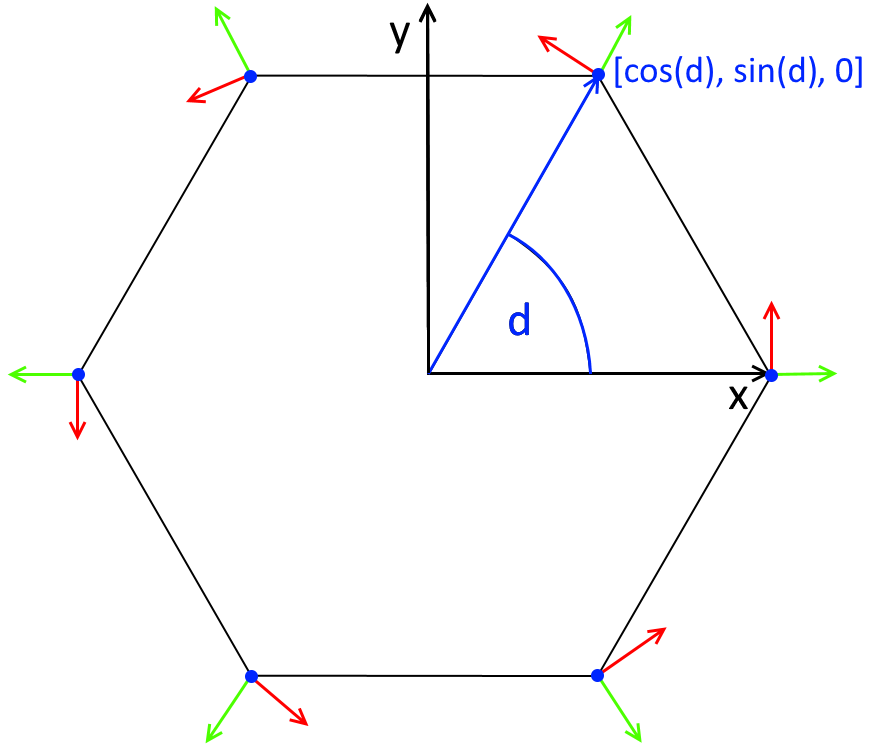
\includegraphics[height=0.25\textheight]{images/Ring6Sections.png}
	\caption{Beispiel für die Berechnung von Vertexpositionen auf einem Einheitskreis mit einer Genauigkeit von sechs Segmenten. $d = \frac{360\degree}{6} = 60 \degree$. Die blauen Punkte entsprechen den Positionen, die grünen Pfeile den Normalen und die roten Pfeile den Tangenten der Vertizes. Eigene Abbildung.}
	\label{fig:Ring6Sections}
\end{figure}
\paragraph{Verbindung der Kreise}
Um den Zylindermantel eines Astsegments zu bilden, werden zwei Kreise mithilfe der Start- und Enddaten des Objekts generiert. Jedes Segment eines Kreises wird mit dem entsprechenden Segment des anderen Kreises verbunden und bildet dadurch ein Zylindersegment. Ein Zylindersegment entspricht somit einem Rechteck. Da das Modell jedoch Dreiecksdaten benötigt, wird jedes Rechteck, wie in Abbildung \ref{subfig:Zylinder10SegmenteWireframe} dargestellt, aus zwei Dreiecken gebildet. \cite{ModelingByNumbersZylindersA:13}
\begin{figure} [hbtp]
\centering
\begin{subfigure}[t]{.4\textwidth}
	\centering
	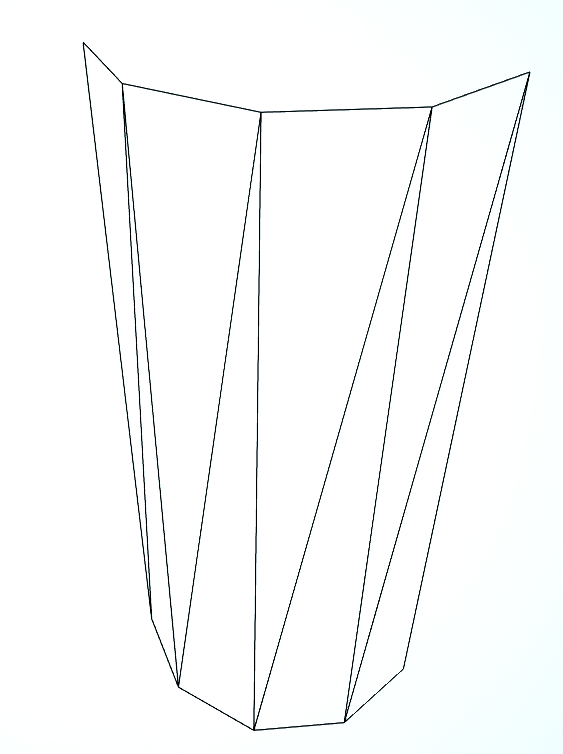
\includegraphics[height=.75\linewidth]{images/Zylinder10SegmenteWireframe.png}
	\caption{Darstellung der Dreiecke, welche bei der Verbindung der Kreise entstehen.}
	\label{subfig:Zylinder10SegmenteWireframe}
\end{subfigure}
\hspace{.1\textwidth}
\begin{subfigure}[t]{.4\textwidth}
	\centering
	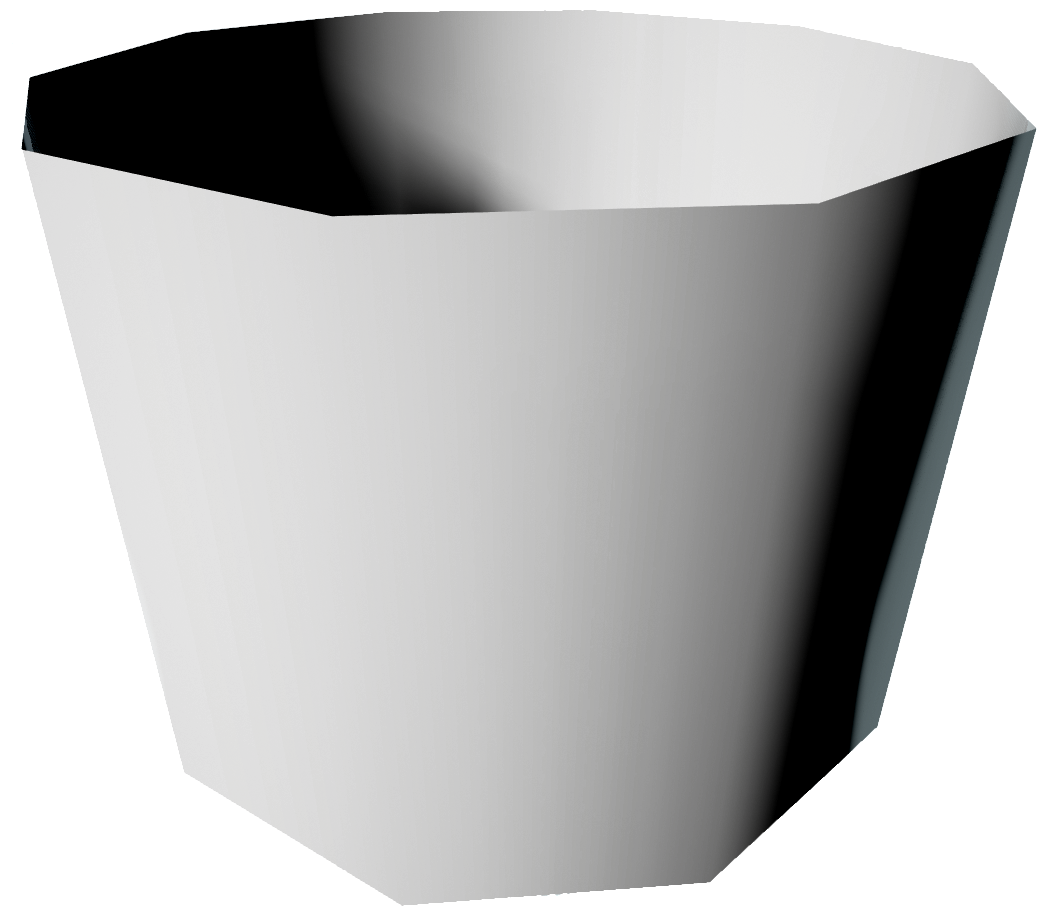
\includegraphics[height=.75\linewidth]{images/Zylinder10SegmenteOpaque.png}
	\caption{Gefärbte Dreiecke mit Beleuchtungsberechnung.}
	\label{subfig:Zylinder10SegmenteOpaque}
\end{subfigure}
\caption{Verbindung zweier Kreise zu einem Zylindermantel. Eigene Abbildungen.}
\label{fig:Zylinder10Segmente}
\end{figure}

Wird jedes Astsegment durch die Verbindung von genau zwei Kreisen dargestellt, führt dies zu der Generierung redundanter Vertexdaten. Die Enddaten eines Astsegments und die Startdaten seines Nachfolgers entsprechen einander, da die daraus generierten Kreis-Vertizes genau aufeinander liegen. Anstatt nun vier Kreise für die Generierung zweier Zylinder zu verwenden, können die Vertizes des verbindenden Kreises wiederverwendet werden -- somit sind drei Kreise für die Generierung zweier Zylinder ausreichend.

Die Verbindung der Modelldaten kann für alle Astsegmente durchgeführt werden, deren Nachfolger dieselbe Zweigtiefe besitzen und somit eine Folge von zusammenhängenden Zylindermodellen bilden. Für einen Nachfolger mit einer sich unterscheidenden Zweigtiefe wird eine neue Folge von zusammenhängenden Zylindermodellen begonnen. \cite{ModelingByNumbersZylindersA:13}

Ein Beispiel für die Generierung zweier Zylinder mithilfe von drei Kreisen wird in Abbildung \ref{subfig:MultiZylinder10SegmenteWireframe} dargestellt.

\begin{figure} [hbtp]
	\centering
	\begin{subfigure}[t]{.4\textwidth}
		\centering
		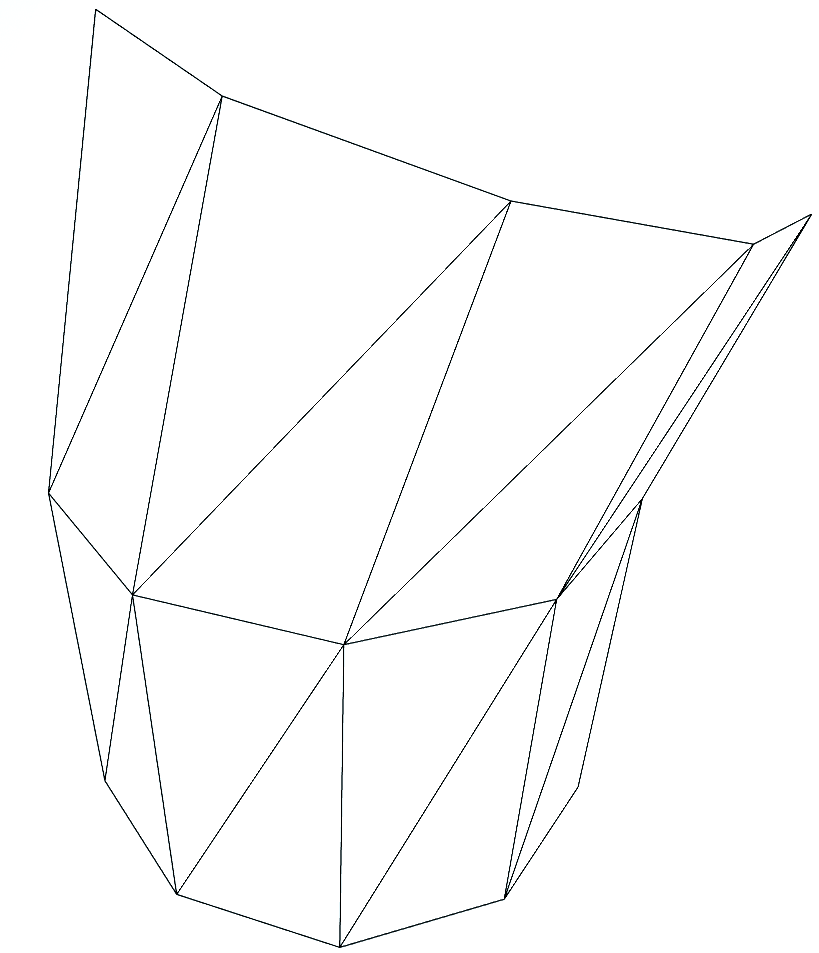
\includegraphics[height=\linewidth]{images/MultiZylinder10SegmenteWireframe.png}
		\caption{Darstellung der Dreiecke, welche bei der Verbindung der Kreise entstehen.}
		\label{subfig:MultiZylinder10SegmenteWireframe}
	\end{subfigure}
	\hspace{.1\textwidth}
	\begin{subfigure}[t]{.4\textwidth}
		\centering
		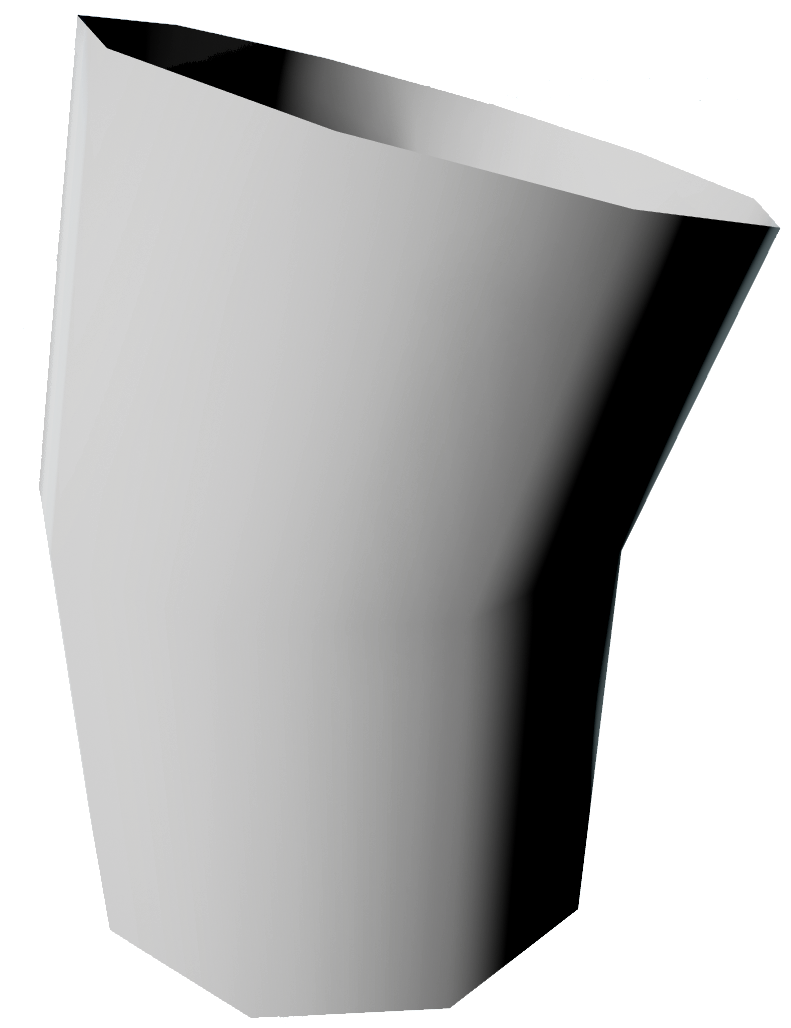
\includegraphics[height=\linewidth]{images/MultiZylinder10SegmenteOpaque.png}
		\caption{Gefärbte Dreiecke mit Beleuchtungsberechnung.}
		\label{subfig:MultiZylinder10SegmenteOpaque}
	\end{subfigure}
	\caption{Verbindung dreier Kreise zu einer Folge zusammenhängender Zylindermodelle. Eigene Abbildungen.}
	\label{fig:MultiZylinder10Segmente}
\end{figure}




